
For all of our analysis we pre-process colour images images into black and white
images. To do this we first remove the blue grid lines from the image and
replace them with white. We then remove all colour information from the image
and resize it such that every cell of the grid is 75 pixels by 75 pixels.

\begin{figure}[h]
    \begin{center}
    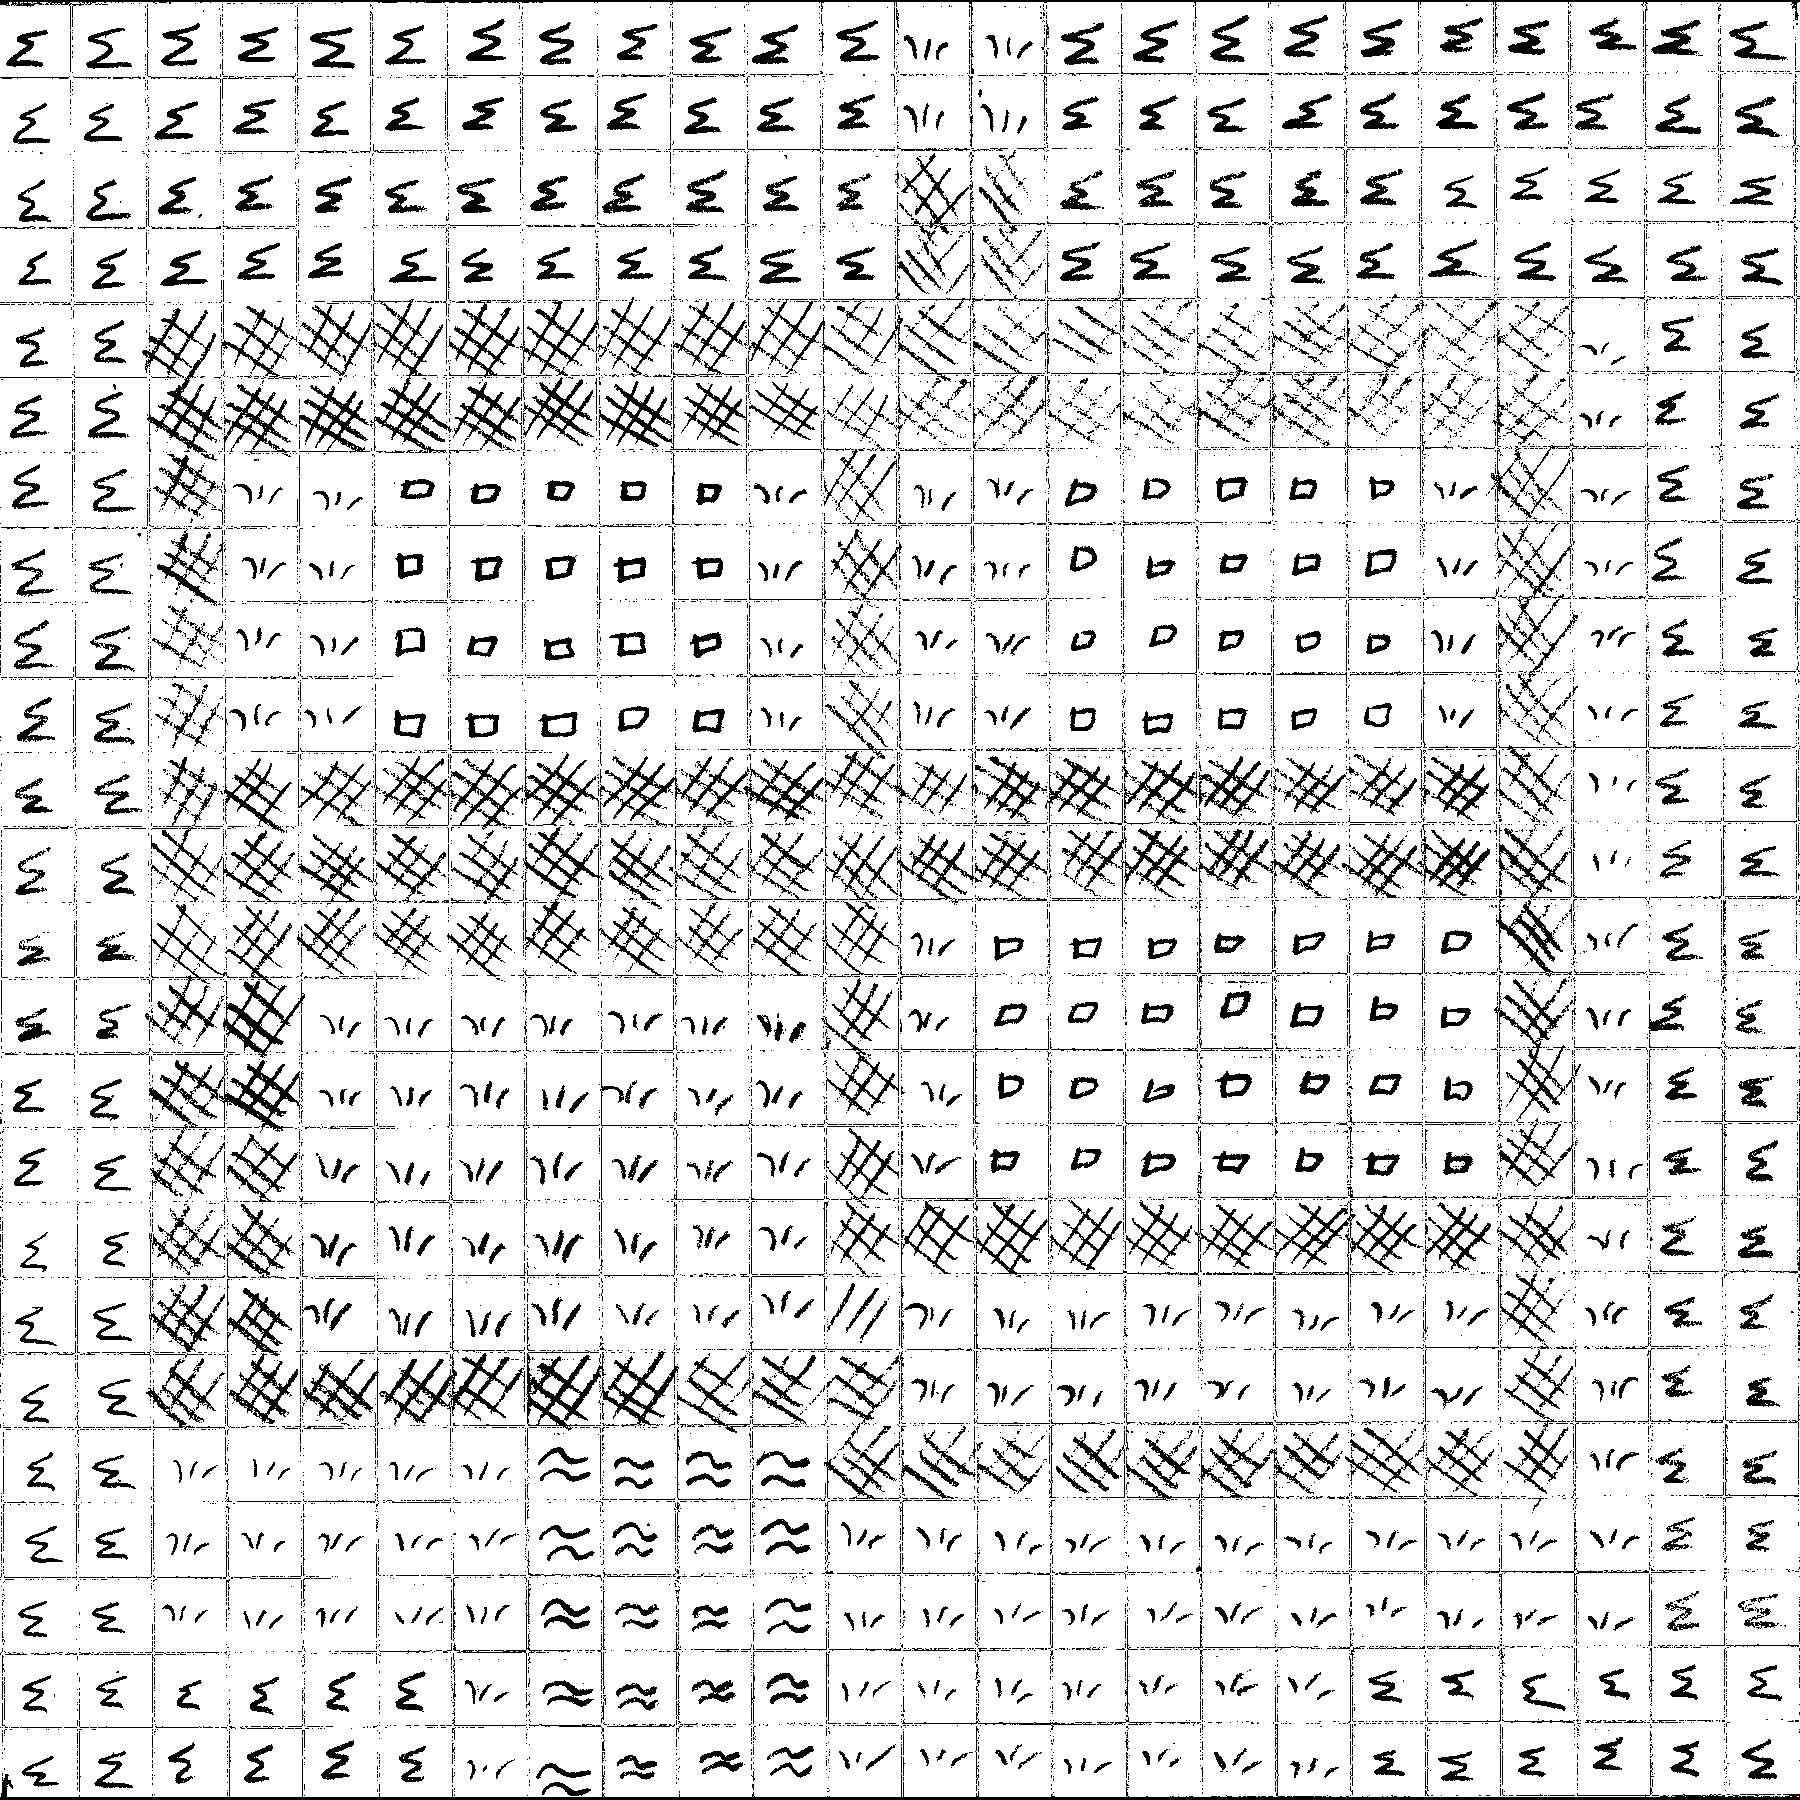
\includegraphics[width=7.5cm, height=7.5cm]{preprocessing-initial}
    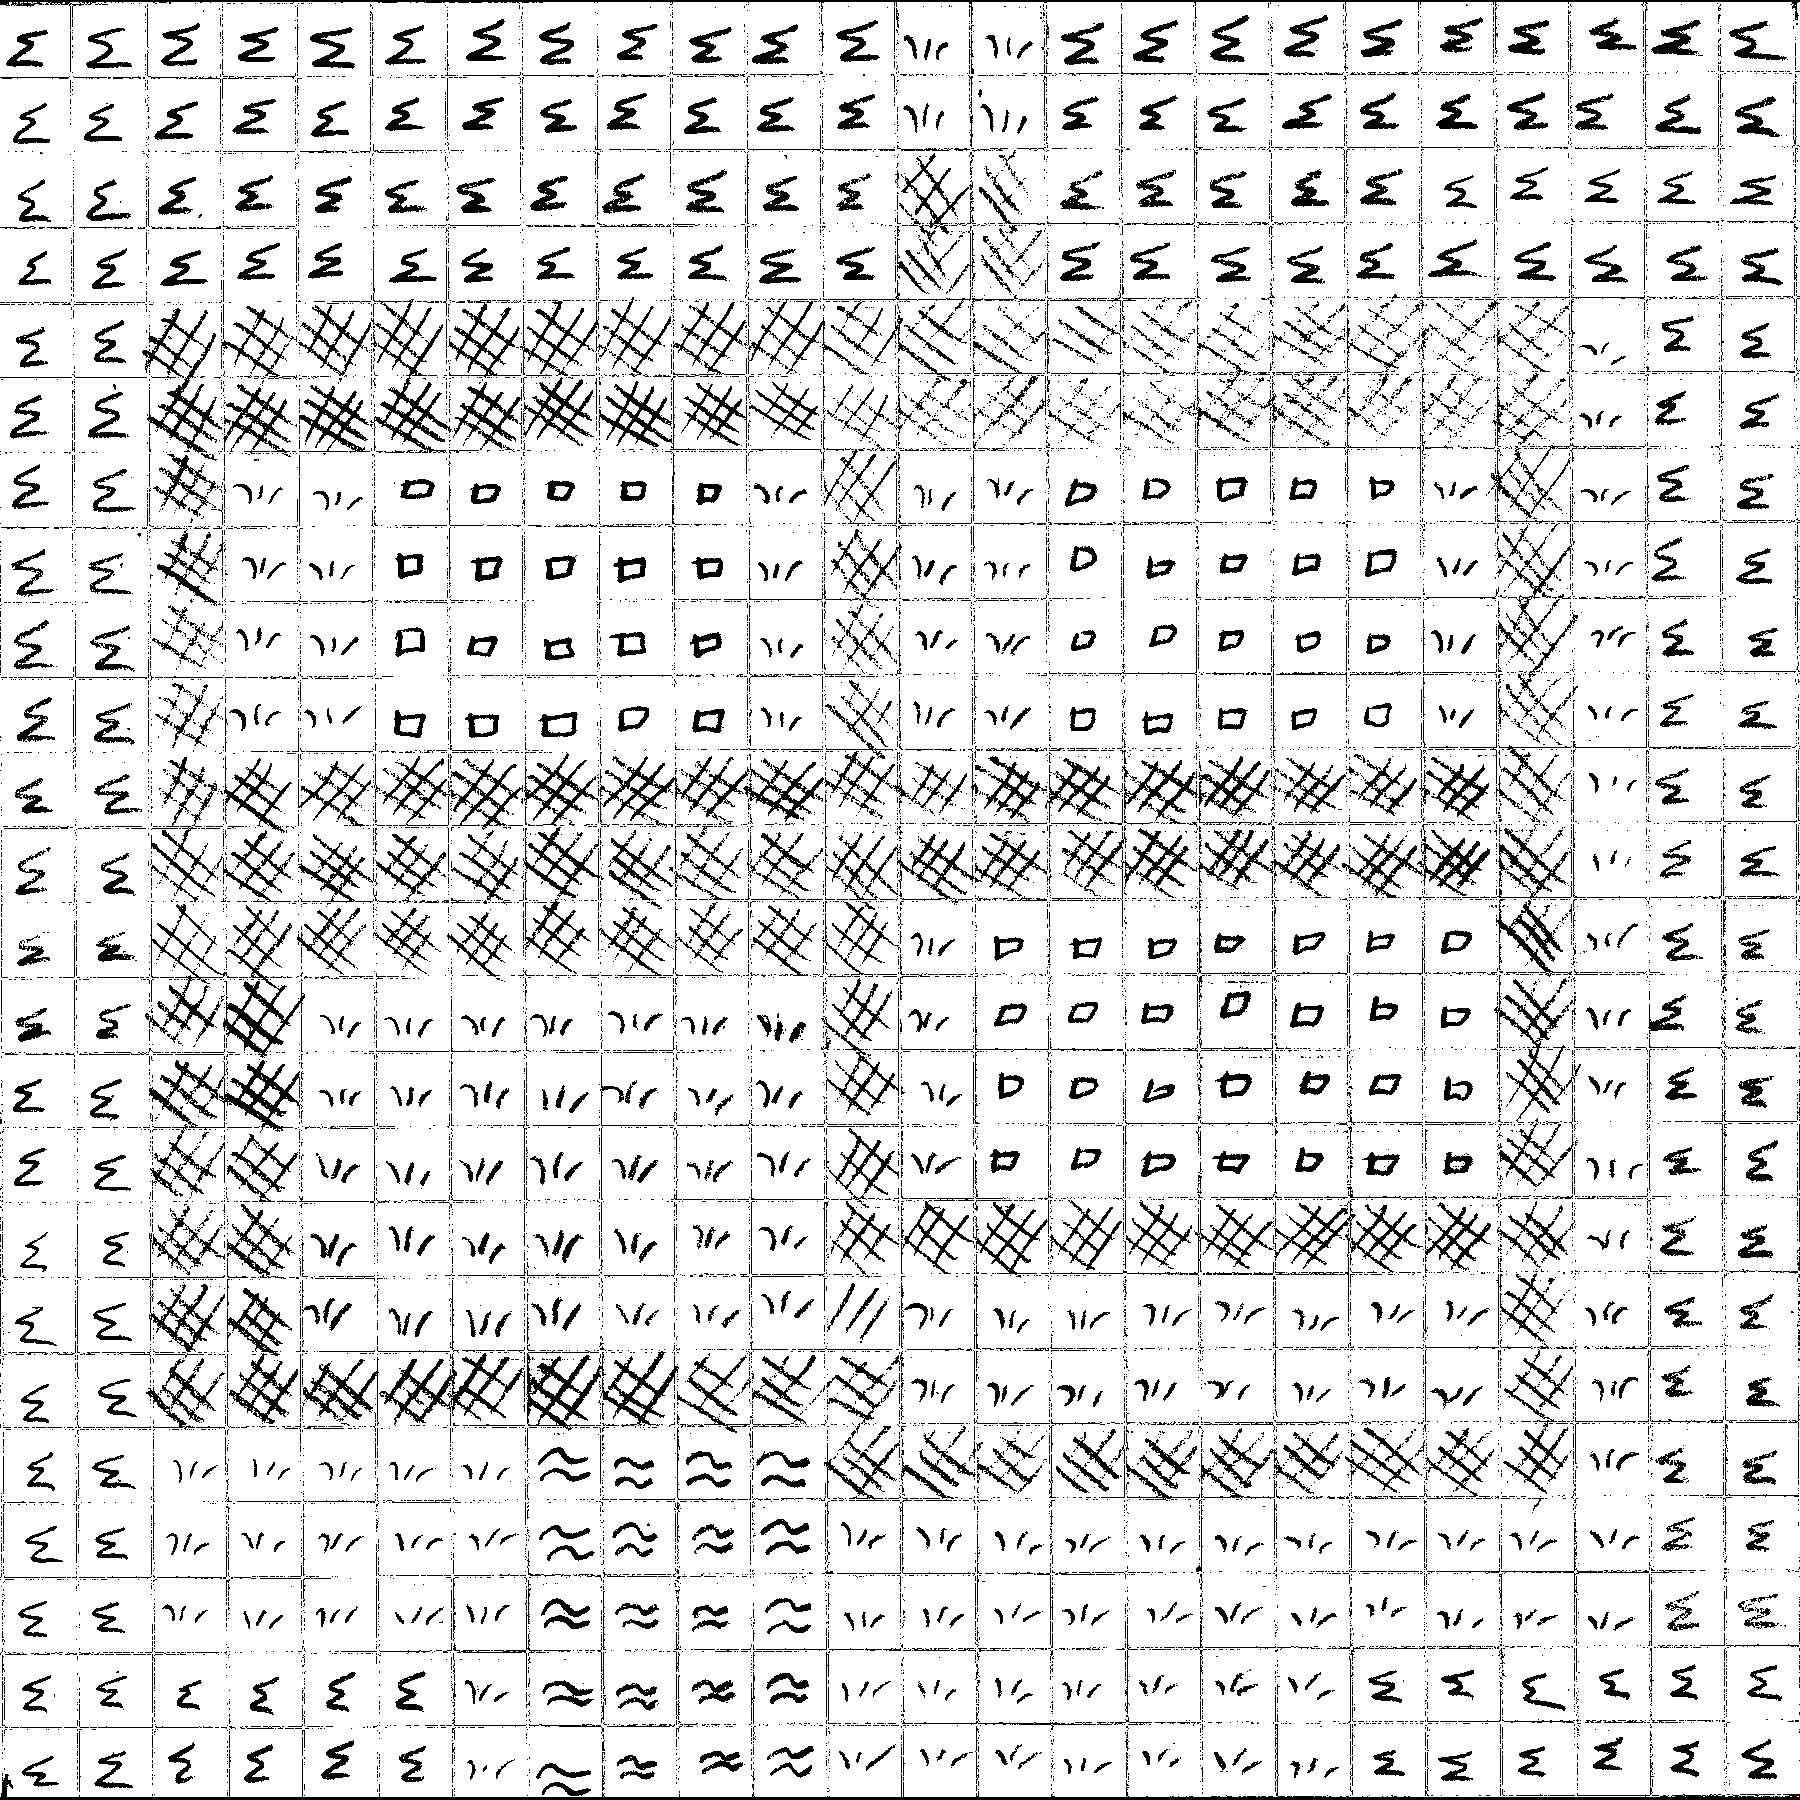
\includegraphics[width=7.5cm, height=7.5cm]{preprocessing-final}

    \caption{Image before preprocessing and image after preprocessing. Notice
        that the contrast has increased and the blue lines have been partially
        removed}

    \end{center}
\end{figure}
